%!TEX root = thesis.tex
\chapter{Discussion}\label{chap:discussion}
\thispagestyle{plain}

    % The discussion is the interpretation and evaluation of the results. It is a
    % comparison of your results with previous findings. It provides the answer to
    % the scientific questions raised in the introduction. It is the "nerve center"
    % of a thesis, whereas the chapter Results may be seen as the "heart".

    % Clearly separate between your own contributions and those of others. Provide
    % rigorous citations of appropriate sources! Explicitly refer to specific 
    % results presented earlier. A certain amount of repetition is necessary. Order
    % discussion items not chronologically but rather logically.

    % The chapter Results answers the question: What has been found? (Facts). The
    % chapter Discussion answers the question: How has the  result to be interpreted?
    % (Opinion).

    % The most important message should appear in the first paragraph. The answer to
    % the key question may appear in the first sentence: e.g., did your original idea
    % work, or didn't it? The following questions may be answered in the discussion
    % section:
    % - Why is the presented method simpler, better, more reliable than previous
    % ones?
    % - What are its strengths and its limitations?
    % - How significant are the results?
    % - How trustworthy are the observations?
    % - Under which conditions and for which region are the results/method valid?
    % - Can the results be easily transferred to other regions or fields?

    The \vas{} model is able to simulated glaciers under various climate inputs with conceptually correct results.
    The ice volume projections for the Alps and High Mountain Asia over the 21st century show that the \vas{} model produces results in agreement with recent studies \citep[e.g.,][]{Marzeion2020}. Despite the lack of a dedicated ice physics module, the projected changes in relative ice volume are comparable to the flowline model---even if not always within its uncertainty bounds. More precisely, the changes in glacier geometries estimated by the \vas{} model are generally smaller than those of the flowline model. The limitations of the \vas{} model responsible for the differences are identified with idealized equilibrium experiments: the missing mass-balance-elevation feedback causes symmetric results for positive and negative mass balance perturbations; the response time scaling results in an oscillating behavior, paradoxically caused by too long model-internal time scales, while the resulting response time scales are rather short. This chapter discusses strength and limitations of the \vas{} model and frames its performance in relation to other models and recent studies.
    
    \section{Values of ice volume (change)} % (fold)
    \label{sec:relative_and_absolute_values_of_ice_volume_change}

        Using the \vas{} relation to estimate initial glacier ice volumes results in much lower values compared to the numerical ice thickness inversion \citep[cf.][]{Farinotti2009} used by the OGGM flowline model. However, comparing the initial ice volumes for the Alps (see Section~\ref{sec:regional_runs_with_all_alpine_glaciers_results}) to the consensus estimate of 130\SI{\pm30}{\cubic\kilo\meter} for Central Europe (RGI region 11) by \citet{Farinotti2019}, the \vas{} model estimate of \SI{130}{\cubic\kilo\meter} is much closer than the flowline model estimate of \SI{164}{\cubic\kilo\meter}. This overestimation of the flowline model is mainly a result of the fixed default values for the ice creep parameter $A$ and the sliding parameter $f_s$. The effect of $A$ on the ice volume estimation on the example of Hintereisferner is shown in \citet[Figure 6]{Maussion2019}, with similar results as presented in Table~\ref{tab:hintereisferner_equilibrium_values}. Calibration of $A$ with ice thickness observations suggest a correction of $A$ with a factor of 1.1 to 1.5 on the global scale, and even more on a regional scale, e.g., a factor 3 for the Alps \citep{OGGM-pitfalls}. Since these parameters are also used for the forward dynamical model run, they do not only affect the initial volume estimations but also ice volume change estimations.

        Stepping away from the idealized equilibrium experiments, how do the ice volume projections over  the 21st century for Central Europe (Section~\ref{sec:projections_for_the_21st_century}) compare to the literature? \citet[cf. Figure 21]{Marzeion2012b} estimate a total ice loss of $\SI{-48}{\percent} \equiv \SI{0.12}{\milli\meter\sealevelrise}$ for RCP2.6, $\SI{-65}{\percent} \equiv \SI{0.16}{\milli\meter\sealevelrise}$ for RCP4.5, $\SI{-69}{\percent} \equiv \SI{0.18}{\milli\meter\sealevelrise}$ for RCP6.0, $\SI{-85}{\percent} \equiv \SI{0.22}{\milli\meter\sealevelrise}$ for RCP8.5 relative to 2020 (reconstructed from supplementary material). These values are quite comparable but slightly higher than estimated by the \vas{} model under comparable SSPs. Possible explanations include the following: the use of CMIP5 data for the entire run, i.e., also for the historical part up to 2012, instead of CRU data; the different mass balance calibration parameters, and the usage of the precipitation gradient. However, the results of \citet{Marzeion2012b} could not fully be reproduced to by the new implementation of the \vas{} model. This would warrant further investigations and a direct comparison using the original code.

        All other recent studies using different models to run global projections under CMIP5 present generally higher values of ice loss for Central Europe than the \vas{} model:
        \citet{Radic2014a} estimate \SI{-84}{\percent} for RCP4.5 and \SI{-96}{\percent} for RCP8.5 (relative to 2006); \citet{Huss2015} estimate \SI{-77}{\percent} for RCP2.6, \SI{-89}{\percent} for RCP4.5 and \SI{-98}{\percent} for RCP8.5 (relative to 2010); \citet{Zekollari2019} estimate \SI{-63}{\percent} for RCP2.6, \SI{-78}{\percent} for RCP4.5 and \SI{-94}{\percent} for RCP8.5 (relative to 2017). Hereby, all values refer to the respective ensemble means. The results from the flowline model are somewhere in between these values. The same general remarks hold true for the projections for High Mountain Asia. A complete comparison of 21st century projection results for all RGI regions and eleven global models is shown in \citet[Figures S1--S20 in the supporting informations]{Marzeion2020}. 

        As a final note, for the \vas{} model it is possible to adjust the absolute values of initial ice volume by using regionally calibrated scaling parameters. However, the sensitivity analysis (Section~\ref{sec:sensitivity_to_scaling_parameters_results}) shows that the relative volume change is not affected by different parameters (in agreement with \citet{Radic2007, Radic2008}). The missing processes that were identified in this study are discussed in the following section.
    
    % section relative_and_absolute_values_of_ice_volume_change (end)

    \section{Missing physical processes} % (fold)
    \label{sec:missing_physical_processes}
    
        The positive feedback loop between surface mass balance and surface elevation has a non-negligible effect on glacier mass change \citep{Huss2012a, Schafer2015}. If the surface elevation decreases as a result of a negative mass balance, the air temperature above the ice surface will subsequently increase, according to the negative temperature gradient. Higher temperatures, in turn, lead to increased melt, which further decreases the surface elevation (this feedback loop works analogously for increasing surface elevations due to positive mass balance). However, the only direct feedback between glacier geometry and specific mass balance of the \vas{} model happens at the glacier terminus.
        Changes in glacier length are linearly relayed to changes in terminus elevation, depending on the average surface slope. This is aggravated with the fact that the modeled changes in glacier length are strongly underestimated, which results in a general underestimation of glacier mass change and a symmetric response to positive and negative step changes in temperature. The symmetric response can be reproduced by the flowline model, if the implemented mass-balance-elevation feedback is turned off (see Section~\ref{sec:single_glacier_test_case_results},~\ref{sec:regional_runs_with_all_alpine_glaciers_results}).

        The missing implementation of explicit thickness changes additionally influences the change of glacier length. \citet{Roe2014} show that glaciers respond to step changes in climate in three overlapping stages:
        \begin{enumerate*}[label=(\arabic*)]
            \item changes in interior thickness cause
            \item changes in terminus flux, which in turn drive
            \item changes in glacier length.
        \end{enumerate*}
        Subsequently, the glacier length does not change exponentially, but much rather sigmoidally. The length change rate needs some time to ramp up to its maximum value, before it slowly drops again and the glacier length approaches its new equilibrium value. The third-order linear ARMA(3,3) model proposed by \citet{Roe2014} is able to adequately simulate all three stages. It produces a sigmoidal change of glacier length, and performs comparably to a flowline model.

        % Different results for attribution: Roe et al. (2020) vs Marzeion et al. (2014)
        % Time scales too long
        Using this three-stage model, \citet{Roe2020} attribute all of the observed glacier mass loss over the industrial era to anthropogenic forcings. This disputes the findings of \citet{Marzeion2014a}, who estimated an anthropogenic contribution of only 25\SI{\pm35}{\percent} during the period from 1851 to 2010 increasing to 69\SI{\pm24}{\percent} over the last twenty years (1991--2000) using the \vas{} model. A possible explanation can be found in the model-internal time scales. The model-internal time scale for length changes used by \citet{Marzeion2012b} is based on the mass turnover $\tau_L \propto 1/P^\text{solid}_\text{clim}(t^*)$ (see Section~\ref{sub:glacier_evolution_model} for details), rather than using the geometric timescale $\tau_L \propto -1/\dot{b}_\text{terminus}$ proposed by \citet{Johannesson1989}. \citet{Roe2020} argue that the computed response times are too large, since the average precipitation is mostly lower than the corresponding terminus ablation rate. This corroborates the findings presented in Section~\ref{sec:sensitivity_to_model_internal_time_scales_results}. The oscillatory behavior of the geometry response can be reduced by lowering the model internal time scales. However, the \vas{} already shows strong short term variability under natural year-to-year climate variability. Lowering the model-internal time scales may result in even stronger fluctuations and make the model react even quicker to changes in climate.

        % ACF vs. response time scales
        The widely used e-folding response time scale can not be linked directly to any glacier characteristic and should be seen as a relative measure much rather than an absolute number \citep{Schuster2020}. The ACF could possibly add information, or even supersede, to the concept of e-folding response times as glacier characteristics.  Possible future work could include a in-depth investigation on how glacier characteristics influence its ACF.
 
    % section missing_physical_processes (end)
    
    

    \section{Mass balance calibration} % (fold)
    \label{sec:mass_balance_calibration}

        % An additional argument brought up by \citet{Roe2020} concerns the mass balance calibration method.
        \citet{Roe2020} additionally argue that the mass balance calibration is another source of uncertainty. By assuming that neighboring glaciers are likely in equilibrium around the same time only climatic factors are considered, while other factors, like the glacier size, are neglected. Small glaciers (or more precisely, glaciers with a short response time) are never far from equilibrium due to their fast geometry adjustments, while large glaciers (or more precisely, glaciers with a long response time) may take many years before they even start reacting to a trend in climate. This potential source of uncertainty is already acknowledged by \citet{Maussion2019}, reasoning that even potentially large errors in \tstar{} will result in comparably small errors in \mustar{}, due to the equilibrium constraint. However, an investigation of this problem is not possible within this study, since the \vas{} model and the OGGM both rely on the same calibration method and are therefore equally affected by it.

        % Sum over monthly average vs. average over yearly sum
        A different problem with the mass balance calibration presents by \citet{Marzeion2012b} concerns the difference between summing over monthly averages versus the averaging over yearly sums for the climatological value of melting temperature.
        Using monthly climatological values (as in the average temperature in January) has a potential pitfall. Imagine a hypothetical time series of average January temperatures over 31 years, with an average monthly temperature  around \SI{-10}{\celsius} for each year except one particularly warm year with \SI{+10}{\celsius}. The climatological temperature average for January will therefore be close to \SI{-10}{\celsius}. Hence, using this monthly average for the mass balance calibration no melt occurs in January. But that one warm January with a highly positive temperature has definitely caused some ice melt, which is not accounted for by the climatological value. Therefore the use of yearly sums of positive melting temperature and solid precipitation, so the mass loss and mass gain of each month is accounted for. However, this problem was already identified and implemented in the OGGM.
    
    % section mass_balance_calibration (end)

    \section{Initializing historic glacier states} % (fold)
    \label{sec:initializing_historic_glacier_states}

        % Start area finding problem.
        The initialization of past glacier states proposed by \citet{Marzeion2012b}, or much rather the implementation thereof, has a conceptual error. Response time scaling introduces a ``glacier memory'', which inhibits the model to run backwards in time. Hence, the value for the initial glacier surface area in 1850 (the year in which the original historic simulations started) is estimated via a trail-and-error process: iterating over a range of possible values for the 1850 area and choosing the one which results in the area closest to the RGI observation at the year of measurement\footnote{Implementation note: the task \lstinline`find_start_area()` uses a minimization function rather the originally described and used iterative process and it allows to decide whether to update the terminus elevation or not.}.

        % Figure showing Hintereisferner time series plots - on page
        \begin{figure}[ht]
          \centering

          % original impelementation
          \begin{subfigure}[b]{0.3\textwidth}
            \caption{Original implementation with constant (i.e., not adjusted) initial terminus elevation}
            \label{fig:start_area:original}
            \centering
            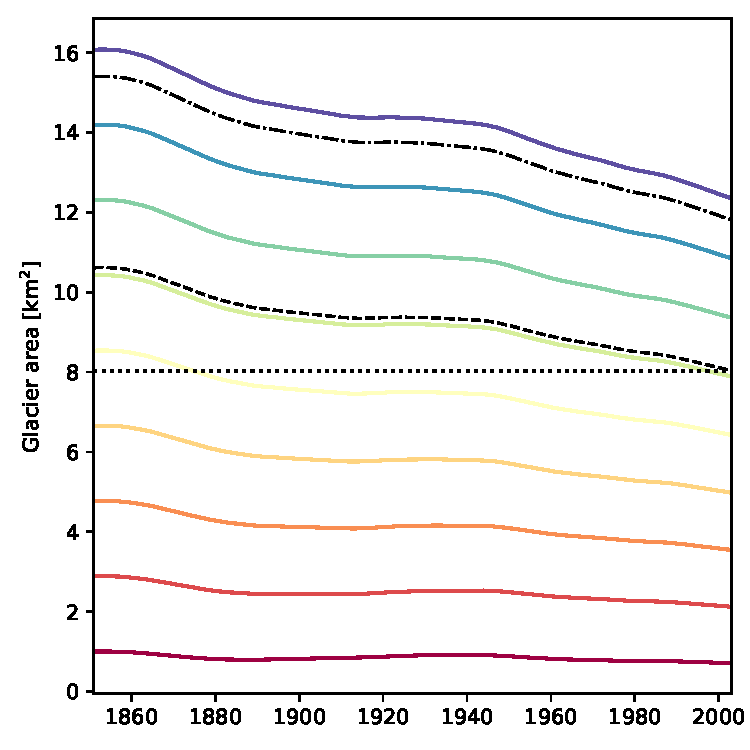
\includegraphics[width=\textwidth]{../plots/start_area/RGI60-11.00897_original.pdf}
          \end{subfigure}
          \hfill
          % my implementation
          \begin{subfigure}[b]{0.3\textwidth}
            \caption{Physical consistent implementation with adjusted initial terminus elevation}
            \label{fig:start_area:overturn}
            \centering
            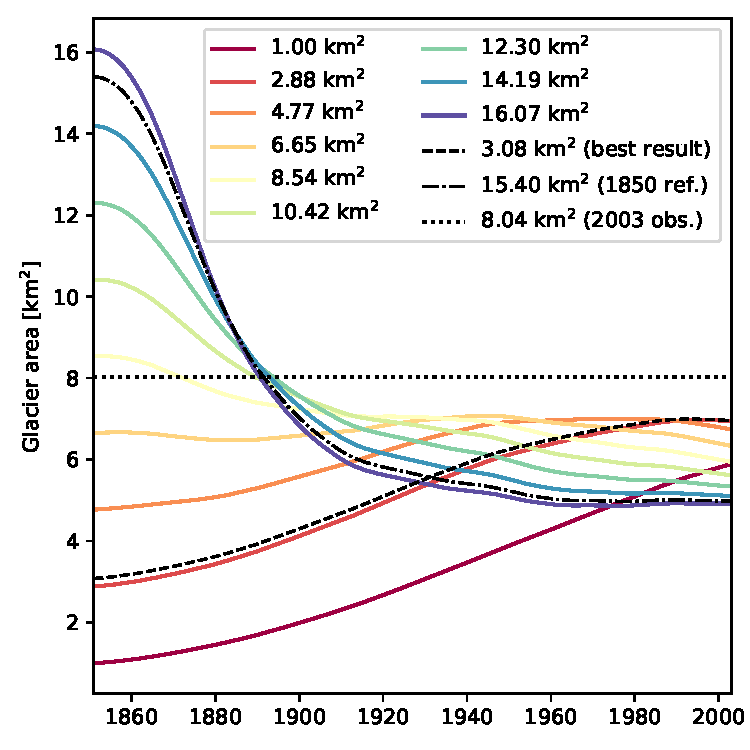
\includegraphics[width=\textwidth]{../plots/start_area/RGI60-11.00897_overturn.pdf}
          \end{subfigure}
          \hfill
          % instant update
          \begin{subfigure}[b]{0.3\textwidth}
            \caption{Physical consistent implementation with added instant geometry changes, i.e., $\tau_L = \tau_A = \SI{1}{\year}$}
            \label{fig:start_area:instant}
            \centering
            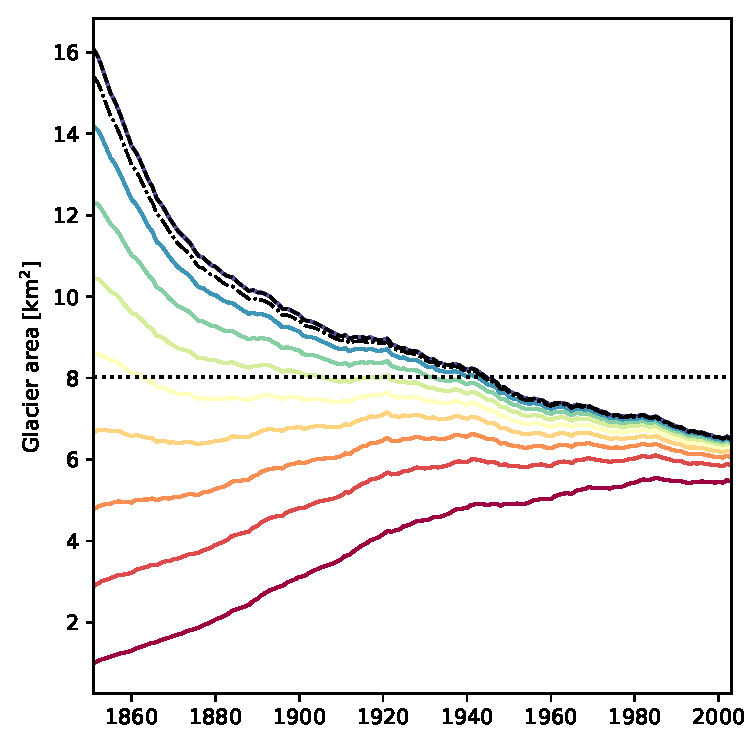
\includegraphics[width=\textwidth]{../plots/start_area/RGI60-11.00897_instant.pdf}
          \end{subfigure}
          
          \caption{Evolution of Hintereisferner (RGI60-11.00897) surface area for different initial values, from 1851 to 2003, forced by HISTALP climate data.}
          \label{fig:start_area}
        \end{figure}

        % original
        Figure~\ref{fig:start_area:original} shows the result  of this process, i.e., the temporal evolution of glacier surface area from 1850 to 2003 for different start values on the example of Hintereisferner. For each iteration, the initial volume $V_0$ and initial length $L_0$ are estimated from the initial area $A_0$ using the scaling relations (see Section~\ref{sub:glacier_evolution_model} and Figure~\ref{fig:iteration-scheme}). The terminus elevation, however, is not adjusted to the new glacier length, but kept constant at the RGI reference value. Thereby, the new and now larger (or smaller) glacier is confined to the same elevation band as the RGI reference glacier, which implies a lower (or higher) average slope. This may make intuitive sense, given the Alpine topography of steep mountains and flatter valleys, and also the results do not look suspicious (which is probably why the bug was not noticed). However, keeping the initial terminus elevation constant results in equal initial specific mass balance for different sized glaciers, which makes little physical sense.

        % fix - overturn
        This problem is easily fixed by adjusting the terminus elevation to the new glacier length, in the same way as during all the other time steps (see Section~\ref{sub:glacier_evolution_model} and Figure~\ref{fig:iteration-scheme}). This results in higher and mostly positive values of initial specific mass balance for smaller initial glaciers (given that they retreat into higher elevations), and lower and possibly negative values for larger initial glaciers (given that they reach further into the ablation zone). However, by doing so, the model is not able to reproduce a surface area close to the observed area in 2003 for some glaciers, regardless of the initial area in 1850 (see Figure~\ref{fig:start_area:overturn}). Furthermore, the larger initial glaciers end up with a lower surface area than the smaller initial glaciers. This ``turn over'' is also seen for ice volume and glacier length (not shown), and reinforces the notion that the model internal time scales are too long, i.e., past glacier states have too much of an influence.

        % instant geometry update
        The hypothesis of too long time scales is tested by allowing for instant geometry updates, i.e., setting the time scales to $\tau_L = \tau_A = \SI{1}{\year}$. As can be seen Figure~\ref{fig:start_area:instant}, the ``overturning'' vanishes. However, the areas still converge to a similar range as for the physically consistent model, which may in some cases be far off the observed value.

        When comparing the original and physical consistent implementation, the same initial areas, even if only slightly different from the RGI reference value, result in drastically different glacier evolutions (look at $A_0 = \SI{6.65}{\square\kilo\meter}$ and $A_0 = \SI{10.42}{\square\kilo\meter}$ in Figure~\ref{fig:start_area:original}~and~\subref{fig:start_area:overturn}). It hints on a dependency of the time scales to the average slope. This additionally supports the argument that the terminus mass balance is a better suited to estimate glacier time scales than precipitation, since terminus mass balance also depends on the average surface slope, or much rather the terminus elevation.

    % section initializing_historic_glacier_states (end)
    
       
    % TODO -> add to Conclusion

    % Trying to sell the OGGM template module
    % As a final note, the implementation of the \vas{} model in the OGGM framework is a success on its own. As suggested by \citet{Maussion2019}, the implementation of simpler approaches, such as the one presented here, allows to test the benefits of the increased model complexity. Such extension of the OGGM are obviously not limited to simple model, but may as well add more complex processes \citep[e.g., an improved calving parametrization,][]{Recinos2019}. It shows the benefits of an open source, modular, community driven glacier model. Comparing different parametrization and estimating uncertainties are imperative to improve projections of future glacier mass loss and its consequences. The comparison shown here is merely a first step.

    % As already mentioned, the here implemented model can be found in its own \href{https://github.com/OGGM/oggm-vas}{GitHub repository}. While the separation from the OGGM codebase complicates continuous testing and ensuring the consistency of the code, it also ensures correct attribution. For details about contributing or extending the OGGM visit the \href{https://docs.oggm.org/en/latest/add-module.html}{documentation}.
